%%%%%%%%%%%%%%%%%%%%%%%%%%%%%%%%%%%%%%%%%%
%%%%%%%%%%%%%                 %%%%%%%%%%%%
%%%%%%%%%%%%%    EXERCISE 1   %%%%%%%%%%%%
%%%%%%%%%%%%%                 %%%%%%%%%%%%
%%%%%%%%%%%%%%%%%%%%%%%%%%%%%%%%%%%%%%%%%%
\begin{exercise}[Slackness in the Kraft inequality]{An instantaneous code has word lengths $l_{1}, l_{2}, \ldots, l_{m},$ which satisfy the strict inequality
  $\sum_{i=1}^{m} D^{-l_{i}}<1$
  The code alphabet is $\mathcal{D}=\{0,1,2, \ldots, D-1\} .$ Show that there exist arbitrarily long sequences of code symbols in $D^{*}$ which cannot be decoded into sequences of codewords.}
  \begin{proof}
  W.l.o.g., we assume $l_1\le l_2 \le \ldots \le l_m$. Since the coding method is instantaneous, for any coding with the length of $l_i$, there exists no other coding that begins with the $l_i$ corresponding coding. That is to say, if there exists a coding with $l_i$ length, then $D^{l_m-l_i}$ codewords of the $D^{l_m}$ codewords will be decodable. Adding all these decodable words up we have
  \begin{equation}
    \sum_{i=1}^{m} D^{l_m-l_i} = D^{l_m} \sum_{i=1}^{m} D^{-l_i} < D^{l_m}
  \end{equation}
  ,which implies that there exists some prefix words in $D^{l_m}$ that are undecodable. Any arbitrary word that begins with such prefix will be unable to decode into sequence of codewords.
  \end{proof}
  \label{ex1}
\end{exercise}

%%%%%%%%%%%%%%%%%%%%%%%%%%%%%%%%%%%%%%%%%%
%%%%%%%%%%%%%                 %%%%%%%%%%%%
%%%%%%%%%%%%%    EXERCISE 2   %%%%%%%%%%%%
%%%%%%%%%%%%%                 %%%%%%%%%%%%
%%%%%%%%%%%%%%%%%%%%%%%%%%%%%%%%%%%%%%%%%%
\begin{exercise}[Fix-free codes]{ A code is a fix-free code if it is both a prefix code and a suffix code. Let $l_{1}, l_{2}, \ldots, l_{m}$ be $m$ positive integers. Prove that if
  $\sum_{k=1}^{m} 2^{-l_{k}} \leq \frac{1}{2}$
  then there exists a binary fix-free code with codeword length $l_{1}, l_{2}, \ldots, l_{m}$}
  \begin{proof}
  W.l.o.g., we assume $l_1\le l_2 \le \ldots \le l_m$. We prove by induction on $m$.
  
  When $m=1$, the conclusion is trivial.

  We assume that when $m=k-1$, for any increasingly ordered positive integers $l_1,l_2,\ldots,l_{k-1}$, if $\sum_{i=1}^{k-1} 2^{-l_i} \le \frac{1}{2}$, then there exists a binary fix-free code with codeword length $l_1,l_2,\ldots,l_{k-1}$.

  Now let $m=k$. For every particular codeword, in terms of prefix codes, it will occupy the space of $2^{l_m - l_i}$ in the tree, while in terms of suffix codes, it wll also occpy the space of $2^{l_m - l_i}$ in the $2^{l_m}$ nodes. These two sets may overlap, but they will surely be less than $2\times 2^{l_m - l_i}$. Hence for all codewords, we have
  \begin{equation}
    2 \sum_{i=1}^{k} 2^{l_m - l_i} \le 2^{l_m} 
  \end{equation}
  
  
  It follows that $\sum_{i=1}^{k} 2^{-l_i} \le \frac{1}{2}$. By removing $l_k$ we have $\sum_{i=1}^{k-1} 2^{-l_i} < \frac{1}{2}$. By the induction hypothesis, we know that for $l_1,\ldots,l_{k-1}$ lengths of codewords, they can form a set of fix-free codes. Furthermore, the strict less relation tells us that there still remains space for the codeword $l_k$. Hence, the conclusion follows.
  \end{proof}
  \label{ex2}
\end{exercise}

%%%%%%%%%%%%%%%%%%%%%%%%%%%%%%%%%%%%%%%%%%
%%%%%%%%%%%%%                 %%%%%%%%%%%%
%%%%%%%%%%%%%    EXERCISE 3   %%%%%%%%%%%%
%%%%%%%%%%%%%                 %%%%%%%%%%%%
%%%%%%%%%%%%%%%%%%%%%%%%%%%%%%%%%%%%%%%%%%
\begin{exercise}[$\frac{3}{4}$ fix-free codes]{ Prove that when
  $$\sum_{k=1}^{m} 2^{-l_{k}} \leq \frac{3}{4}$$  the conclusion above holds.}
  \begin{proof} The proof here is not complete. We try to solve the problem from two perspectives. The proof idea is based on this paper\footnote{R. Ahlswede and B. Balkenhol and L. Khachatrian. Some properties of Fix-Free Codes}.
    \paragraph{There exists no upper bounds greater than $\frac{3}{4}$.} For any $\frac{3}{4}+\epsilon>\frac{3}{4}$, we choose $k$ such that $2^{-k}<\epsilon$. We construct a list of codelengths with $1$ and $2^{k-2}+1$ $k$s. Then we have
    \begin{equation}
      \sum_{i=1}^{N} 2^{-l_i} = \frac{1}{2}+ 2^{-k} (2^{k-2}+1) = \frac{3}{4}+\epsilon
    \end{equation}

    Our choice of codeword lengths satisfies our assumption, however, with the first codeword with length of 1 as a prefix and suffix, there are at most $2^{k-2}$ words of length $k$, which implies that our choice is invalid, contradiction. 

    \paragraph{The conclusion with $\frac{3}{4}$ holds under some restrictions.} We suppose that for all code lengths, either $l_i = l_{i+1}$ or $2l_i \le l_{i+1}$. We prove that under this restriction the conclusion will hold.

    W.l.o.g., we assume that $l_1 \le l_2 \le \ldots \le l_m$. We prove by induction on $m$. The base case of $m=1$ is trivial.

    Assume that for any $n\le m-1$, with $\sum_{i=1}^{n} 2^{-l_i} \le \frac{3}{4}$ we can construct $n$ different codeword lengths. We prove that this holds for the case of $m$.
    
    Let $m'$ be the largest index $i$ with $l_i < l_{m'}$. By induction hypothesis we can construct a fix-free code $C'$ with the lengths $l_1, \ldots, l_{m'}$. Note for every particular word with length $l_i$, it will occupy at most $2\times 2^{l_{m}-l_i}$ nodes due to the prefix and suffix rule. However, with our restriction, $2^{l_m - 2l_i}$ nodes will be returned, since they will not actually be used as codewords. Therefore, at the $l_m$ level, at most $2 \sum_{i=1}^{m'} 2^{l_m-l_i}- \sum_{i=1}^{m'}2^{l_{m} - 2l_i}$ nodes will be occupied.\footnote{The paper gives a more detailed formula, but I can't fully understand how the last component formula is derived. Fortunately leaving the that component out will not affect the proof here. }

    To ensure that the remaining $l_{m'+1},\ldots,l_m$ can be added to the orginal code system we should have

    \begin{equation}
      2 \sum_{i=1}^{m'} 2^{l_m -l_i}- \sum_{i=1}^{m'}2^{l_m - 2l_i} \le 2^{l_m} - (m -m')
      \label{eqn1}
    \end{equation}

    Writing $K = m - m'$ and $\alpha = \sum_{i=1}^{m'} 2^{-l_i}$. (\ref{eqn1}) can be written as

    \begin{equation}
      2\alpha - \alpha^2 \le 1 - \frac{K}{2^{l_m}}
    \end{equation}

    With abbreviation $\beta = \sum_{i=1}^{m} 2^{-l_i} = \alpha + \frac{K}{2^{l_m}}$ and $\delta = \frac{K}{2^{l_m}}$ we get the equivalent inequality

    \begin{equation}
      \beta \le 1+\delta - \sqrt{\delta}
    \end{equation}

    Note $\delta \in (0,1)$, the right side has the minimal value of $\frac{3}{4}$ at $\delta = \frac{1}{4}$. Thus for any $ \sum_{i=1}^{m} 2^{-l_i} \le \frac{3}{4}$, the conclusion holds.

  \end{proof}
  \label{ex3}
\end{exercise}

%%%%%%%%%%%%%%%%%%%%%%%%%%%%%%%%%%%%%%%%%%
%%%%%%%%%%%%%                 %%%%%%%%%%%%
%%%%%%%%%%%%%    EXERCISE 4   %%%%%%%%%%%%
%%%%%%%%%%%%%                 %%%%%%%%%%%%
%%%%%%%%%%%%%%%%%%%%%%%%%%%%%%%%%%%%%%%%%%
\begin{exercise}[More Huffman codes]{Find the binary Huffman code for the source with probabilities $\left(\frac{1}{3}, \frac{1}{5}, \frac{1}{5}, \frac{2}{15}, \frac{2}{15}\right) .$ Argue that this code is also optimal for the source with probabilities $\left(\frac{1}{5}, \frac{1}{5}, \frac{1}{5}, \frac{1}{5}, \frac{1}{5}\right)$}
  \begin{solution}
    \begin{figure}[H]
      \caption{Huffman Code for $\left(\frac{1}{3}, \frac{1}{5}, \frac{1}{5}, \frac{2}{15}, \frac{2}{15}\right) .$}
      \centering
      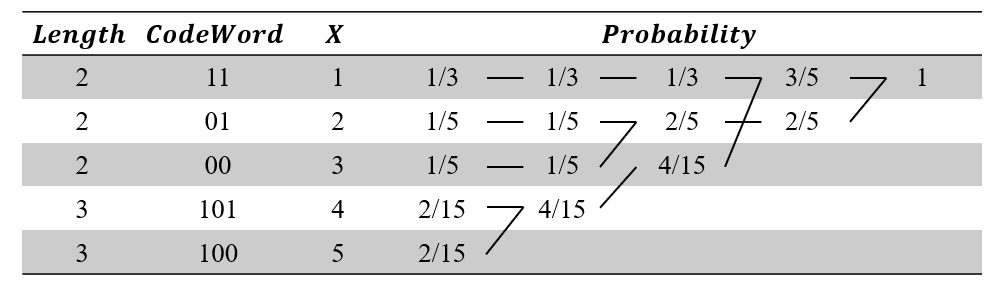
\includegraphics[width=11cm]{img/5-1.png}
      \label{fig:ex4}
    \end{figure}
    The huffman code of  $\left(\frac{1}{3}, \frac{1}{5}, \frac{1}{5}, \frac{2}{15}, \frac{2}{15}\right) .$ is found as Figure \ref{fig:ex4} shows. 

      \begin{figure}[H]
        \caption{Huffman Code for $\left(\frac{1}{5}, \frac{1}{5}, \frac{1}{5}, \frac{1}{5}, \frac{1}{5}\right)$}
        \centering
        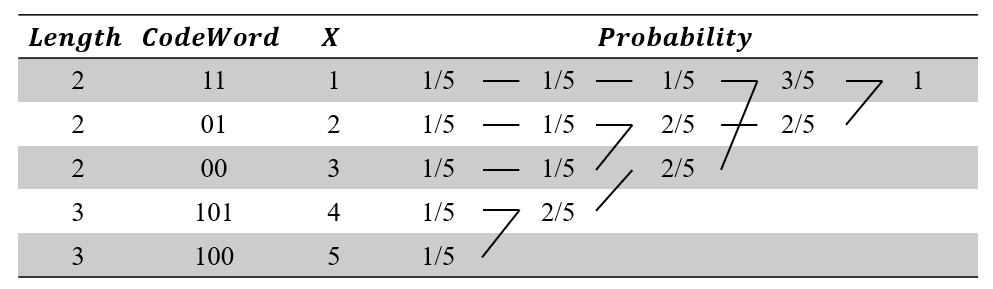
\includegraphics[width=11cm]{img/5-2.png}
        \label{fig:ex5}
      \end{figure}
    We see that for $\left(\frac{1}{5}, \frac{1}{5}, \frac{1}{5}, \frac{1}{5}, \frac{1}{5}\right)$, we can follow an identical process to construct the huffman code, as Figure \ref{fig:ex5} shows. Since huffman code is always optimal, the conclusion holds.
  \end{solution}
  \label{ex4}
\end{exercise}


%%%%%%%%%%%%%%%%%%%%%%%%%%%%%%%%%%%%%%%%%%
%%%%%%%%%%%%%                 %%%%%%%%%%%%
%%%%%%%%%%%%%    EXERCISE 5   %%%%%%%%%%%%
%%%%%%%%%%%%%                 %%%%%%%%%%%%
%%%%%%%%%%%%%%%%%%%%%%%%%%%%%%%%%%%%%%%%%%
\begin{exercise}[Bad codes]{ Which of these codes cannot be Huffman codes for any probability assignment?
  \begin{enumerate}
    \item \{0,10,11\}
    \item \{00,01,10,110\}
    \item \{01,10\}
  \end{enumerate}
  }
  \begin{solution}
  \par{~}
  \begin{enumerate}
    \item { \{0,10,11\} can be the huffman code for distribution $\left\{\frac{1}{2},\frac{1}{4},\frac{1}{4}\right\}$.
    }
    \item { \{00,01,10,110\} can be shortened by \{00,01,10,11\}. It cannot be a huffman code. 

    }
    \item { \{01,10\} can be shortened by \{0,1\}. It cannot be a huffman code.

    }
  \end{enumerate}
  \end{solution}
  \label{ex5}
\end{exercise}

%%%%%%%%%%%%%%%%%%%%%%%%%%%%%%%%%%%%%%%%%%
%%%%%%%%%%%%%                 %%%%%%%%%%%%
%%%%%%%%%%%%%    EXERCISE 6   %%%%%%%%%%%%
%%%%%%%%%%%%%                 %%%%%%%%%%%%
%%%%%%%%%%%%%%%%%%%%%%%%%%%%%%%%%%%%%%%%%%
\begin{exercise}[Huffman 20 questions]{ Consider a set of $n$ objects. Let $X_{i}=$ 1 or 0 accordingly as the $i$ th object is good or defective. Let $X_{1}, X_{2}, \ldots, X_{n}$ be independent with $\operatorname{Pr}\left\{X_{i}=1\right\}=p_{i} ;$ and $p_{1}>$
  $p_{2}>\cdots>p_{n}>\frac{1}{2} .$ We are asked to determine the set of all defective objects. Any yes-no question you can think of is admissible.
  \begin{enumerate}
    \item Give a good lower bound on the minimum average number of questions required. 
    \item If the longest sequence of questions is required by nature's answers to our questions, what (in words) is the last question we should ask? What two sets are we distinguishing with this question? Assume a compact (minimum average length) sequence of questions.
    \item Give an upper bound (within one question) on the minimum average number of questions required.
  \end{enumerate}}
  \begin{solution}
  \par{~}
  \begin{enumerate}
    \item { 
      The asking process can be modeled into the problem of constructing a compressed code for the sequence $X_1,X_2,\ldots,X_n$. The set of all defective objects can be determined if we determine the codeword we've constructed. The question we are asking is a yes-no question, so the codeword is based on a 2-ray alphabet. We can use entropy of $X_1,X_2,\ldots,X_n$ to give a lower bound on the average codeword length.
      \begin{equation}
        \begin{aligned}
          L^* &\ge H_2 (X_1,X_2,\ldots,X_n) \\
          &= \sum_{i=1}^{n} H(X_i) = \sum_{i=1}^{n} H(p_i)
        \end{aligned}
      \end{equation} 
    }
    \item { The longest sequence implies that we are distinguishing between the two least cases in this problem, i.e. the case where all objects are good ($\prod_{i=1}^n(1-p_i)$) and the case where all objects are good except the one that has the least probability to be defective ($p_n \prod_{i=1}^{n-1}(1-p_i)$). The question will be like ``Is $X_n$ defective?''.
    }
    \item { Using the same notion in part 1, the upper bound of the minimum average number of questions (codeword length) will be
    \begin{equation}
      \begin{aligned}
        L^* &\le H_2 (X_1,X_2,\ldots,X_n) + 1 \\
        &= \sum_{i=1}^{n} H(X_i) + 1 = \sum_{i=1}^{n} H(p_i) + 1
      \end{aligned}
    \end{equation}

    }
  \end{enumerate}
  \end{solution}
  \label{ex6}
\end{exercise}

%%%%%%%%%%%%%%%%%%%%%%%%%%%%%%%%%%%%%%%%%%
%%%%%%%%%%%%%                 %%%%%%%%%%%%
%%%%%%%%%%%%%    EXERCISE 7   %%%%%%%%%%%%
%%%%%%%%%%%%%                 %%%%%%%%%%%%
%%%%%%%%%%%%%%%%%%%%%%%%%%%%%%%%%%%%%%%%%%
\begin{exercise}[Simple optimum compression of a Markov source]{Consider the three-state Markov process $U_{1}, U_{2}, \ldots$ having transition matrix

  \begin{table}[H]
    \begin{center}
      \begin{tabular}{c|ccc}
      \diagbox{$U_n$}{$U_{n-1}$} & $S_1$         & $S_2$         & $S_3$         \\ \hline
      $S_1$                                         & $\frac{1}{2}$ & $\frac{1}{4}$ & $\frac{1}{4}$ \\
      $S_2$                                         & $\frac{1}{4}$ & $\frac{1}{2}$ & $\frac{1}{4}$ \\
      $S_3$                                         & 0             & $\frac{1}{2}$ & $\frac{1}{2}$
      \end{tabular}
    \end{center}
    \end{table}

  Thus, the probability that $S_{1}$ follows $S_{3}$ is equal to zero. Design three codes $C_{1}, C_{2}, C_{3}$ (one for each state 1,2 and $3,$ each code mapping elements of the set of $S_{i}$ 's into sequences of 0 's and 1 's, such that this Markov process can be sent with maximal compression by the following scheme: 
  \begin{enumerate}
    \item Note the present symbol $X_{n}=i$
    \item Select code $C_{i}$
    \item Note the next symbol $X_{n+1}=j$ and send the codeword in $C_{i}$ corresponding to $j$
    \item Repeat for the next symbol. 
  \end{enumerate}
  What is the average message length of the next symbol conditioned on the previous state $X_{n}=i$ using this coding scheme? What is the unconditional average number of bits per source symbol? Relate this to the entropy rate $H(\mathcal{U})$ of the Markov chain.
  }
  \begin{solution} We can design the codes using the Huffman method.
    \begin{table}[H]
      \begin{center}
        \begin{tabular}{c|ccc}
          & $S_1$         & $S_2$         & $S_3$         \\ \hline
        $C_1$                                         & 1 & 01 & 00 \\
        $C_2$                                         & 01 & 1 & 00 \\
        $C_3$                                         & N/A             & 0 & 1
        \end{tabular}
      \end{center}
    \end{table}
    We first calculate the stationery distribution of the Markov Chain.
    \begin{equation}
      \left\{\begin{array}{c}
        \mathbf{\mu}P = \mathbf{\mu} \\
        \mathbf{\mu} \mathbf{1}^T = 1
      \end{array}\right. \Rightarrow \mu = \left[\frac{2}{9}, \frac{4}{9},\frac{1}{3}\right]
    \end{equation}
    The average length is
    \begin{equation}
      \sum_{i=1}^{3} \mu_{i} \sum_{j=1}^{3} L(C_{ij}) = \frac{2}{9}\cdot\frac{3}{2} + \frac{4}{9} \cdot\frac{3}{2}+\frac{1}{3}\cdot 1 = \frac{4}{3}
    \end{equation}
    The entropy rate can be calculated as
    \begin{equation}
      H(\mathcal{U})=-\sum_{i j} \mu_{i} P_{i j} \log P_{i j} = \frac{4}{3}
    \end{equation}
    They are the same because the optimal code length is its entropy, which can be expressed with the notion of ``average'' entropy $\frac{1}{n} H(U_1,U_2,\ldots,U_n,\ldots)$, which approximates to $H(\mathcal{U})$.
  \end{solution}
  \label{ex7}
\end{exercise}

%%%%%%%%%%%%%%%%%%%%%%%%%%%%%%%%%%%%%%%%%%
%%%%%%%%%%%%%                 %%%%%%%%%%%%
%%%%%%%%%%%%%    EXERCISE 8   %%%%%%%%%%%%
%%%%%%%%%%%%%                 %%%%%%%%%%%%
%%%%%%%%%%%%%%%%%%%%%%%%%%%%%%%%%%%%%%%%%%
\begin{exercise}[Shannon codes and Huffman codes]{ Consider a random variable $X$ that takes on four values with probabilities $\left(\frac{1}{3}, \frac{1}{3}, \frac{1}{4}, \frac{1}{12}\right)$
  \begin{enumerate}
    \item Construct a Huffman code for this random variable.
    \item Show that there exist two different sets of optimal lengths for the codewords; namely, show that codeword length assignments (1,2,3,3) and (2,2,2,2) are both optimal.
    \item Conclude that there are optimal codes with codeword lengths for some symbols that exceed the Shannon code length $\left\lceil\log \frac{1}{p(x)}\right\rceil$
  \end{enumerate}
}
  \begin{solution}
  \par{~}
  \begin{enumerate}
    \item { A Huffman code is constructed as Figure \ref{fig:ex8-1} shows.
      \begin{figure}[H]
        \caption{Huffman Code for $\left(\frac{1}{3}, \frac{1}{3}, \frac{1}{4}, \frac{1}{12}\right)$}
        \centering
        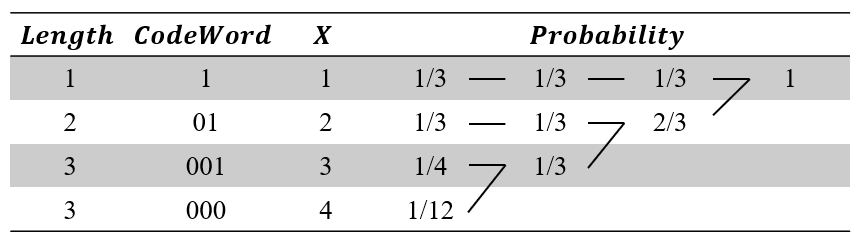
\includegraphics[width=11cm]{img/5-3.png}
        \label{fig:ex8-1}
      \end{figure}
    }
    \item { Another Huffman code is constructed as Figure \ref{fig:ex8-2} shows. They are both optimal for the distribution but with distinct length assignments.
      \begin{figure}[H]
        \caption{Huffman Code for $\left(\frac{1}{3}, \frac{1}{3}, \frac{1}{4}, \frac{1}{12}\right)$}
        \centering
        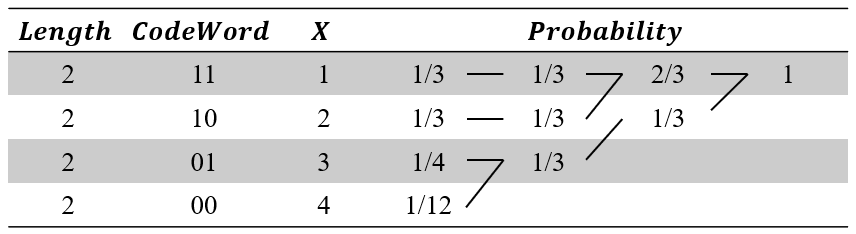
\includegraphics[width=11cm]{img/5-4.png}
        \label{fig:ex8-2}
      \end{figure}
    }
    \item { The case of $X=3$ in Figure \ref{fig:ex8-1} serves as an example. It has the length of 3, exceeding the Shannon length  $\left\lceil\log \frac{1}{p(x)}\right\rceil = 2$. It can be concluded that in some cases, we can construct optimal codes with codeword lengths for some symbols that exceed the Shannon code length.
    }
  \end{enumerate}
  \end{solution}
  \label{ex8}
\end{exercise}

%%%%%%%%%%%%%%%%%%%%%%%%%%%%%%%%%%%%%%%%%%
%%%%%%%%%%%%%                 %%%%%%%%%%%%
%%%%%%%%%%%%%    EXERCISE 9   %%%%%%%%%%%%
%%%%%%%%%%%%%                 %%%%%%%%%%%%
%%%%%%%%%%%%%%%%%%%%%%%%%%%%%%%%%%%%%%%%%%
\begin{exercise}[Data compression]{ Find an optimal set of binary codeword lengths $\left.l_{1}, l_{2}, \ldots \text { (minimizing } \sum p_{i} l_{i}\right)$ for an instantaneous code for each of the following probability mass functions:
  \begin{enumerate}
    \item $\mathbf{p}=\left(\frac{10}{41}, \frac{9}{41}, \frac{8}{41}, \frac{7}{41}, \frac{7}{41}\right)$
    \item $\mathbf{p}=\left(\frac{9}{10},\left(\frac{9}{10}\right)\left(\frac{1}{10}\right),\left(\frac{9}{10}\right)\left(\frac{1}{10}\right)^{2},\left(\frac{9}{10}\right)\left(\frac{1}{10}\right)^{3}, \ldots\right)$
  \end{enumerate}
  }
  \begin{solution} The optimal code is given in Figure \ref{fig:ex9} by the Huffman rule. Note that in problem (2) we have that any probability is greater than the sum of the probabilities less than itself. Hence, we can construct the Huffman code in a monotonous order
  \end{solution}
  \label{ex9}
\end{exercise}

\begin{figure}[htbp]
  \centering
  \caption{Huffman Code for Exercise \ref{ex9}}
      \begin{minipage}[t]{0.95\linewidth}
          \centering
          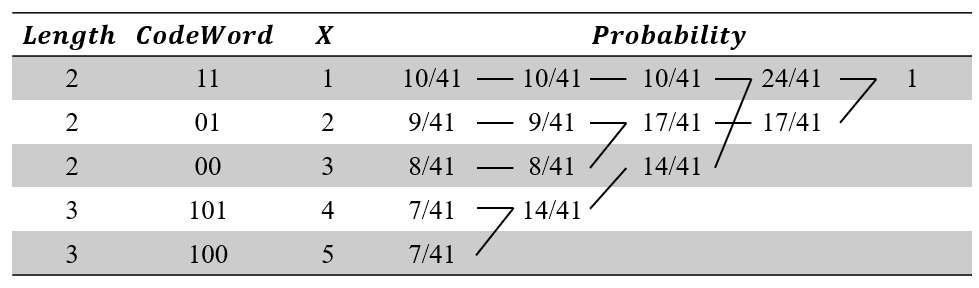
\includegraphics[width=11cm]{img/5-5.png}
      \end{minipage}
      \par{~}
      \begin{minipage}[t]{0.95\linewidth}
          \centering
          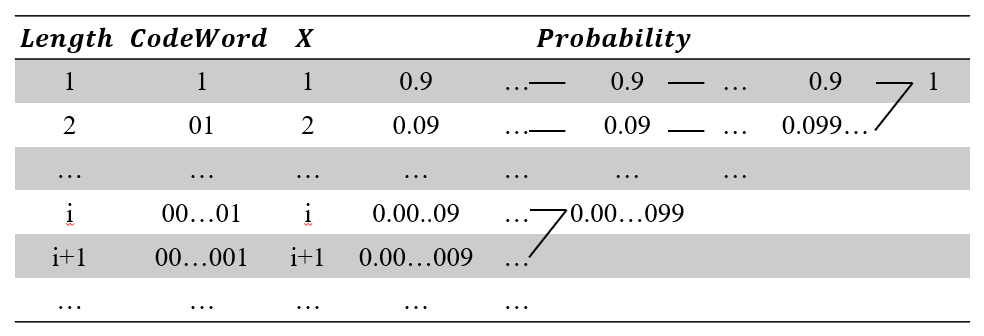
\includegraphics[width=11cm]{img/5-6.png}
      \end{minipage}
    \label{fig:ex9}
\end{figure}

